\documentclass[runningheads,a4paper]{article}
%\documentclass[conference]{IEEEtran}
\usepackage{graphicx}
\usepackage{amsmath}
\usepackage{comment}
\usepackage{amssymb}
\usepackage{xcolor}
\usepackage{caption}
\usepackage{url}
\usepackage[ruled]{algorithm2e}
\usepackage{algorithmic}
%\newtheorem{lemma}{Lemma}
%\newtheorem{theorem}{Theorem}
%\newtheorem{property}{Property}
%\newtheorem{corollary}{Corollary}
%\newtheorem{definition}{Definition}[section]
%\newtheorem{example}{Example}[section]

\title{ Cache Coherence Protocol Design: A Report}
%\author{}
%\institute{}
\newtheorem{definition}{Definition}
\begin{document}

\maketitle
\begin{abstract}
%Industrial Control Systems (ICS) used in manufacturing, power generators
%and other critical infrastructure monitoring and control are  ripe targets for cyber attacks
%these days. Examples of such attacks are abundant such as attacks on Iranian nuclear enrichment plant with Stuxnet in 2009,
%on German steel plant in 2014, Ukrainian power system in 2015 and 2016.
% Usually in ICS, multiple control loops work concurrently and share various resources including the
%communication bus through which they interact with sensors and actuators. Real-time scheduling of concurrent control applications while competing for shared 
%resources demands a delicate balance between performance and real-time constraints.
%A possible insider attack could be the replacement of a previously vetted control application 
%or other components in the system,
%during a system update.  
 [[One  method  of  enforcing  coherence  is  to  ensure  that  a  processor  has  exclusive
 access to a data item before it writes that item. This style of protocol is called a write
 invalidate protocol because it invalidates copies in other caches on a write. Exclusive access
 ensures that no other readable or writable copies of an item exist when the write occurs: 
 all other cached copies of the item are invalidated.-]]--Patterson, page 468.

 bus{\_}invalidate: when a core gets a write hit in its local cache(L1) on shared block,
     then it broadcats a bus{\_}invalidate requests, to inform 
other cores that it has updated the block, other core must invalidate their copy.
 If the core has the data in Modified state, then it can update the data, due to 
Single Write Multiple Read principle, onle one core can have data in Modified state.
 So, if the current core has the data in Modified state, no request should be put
for invalidation.



\begin{figure}
\begin{center}
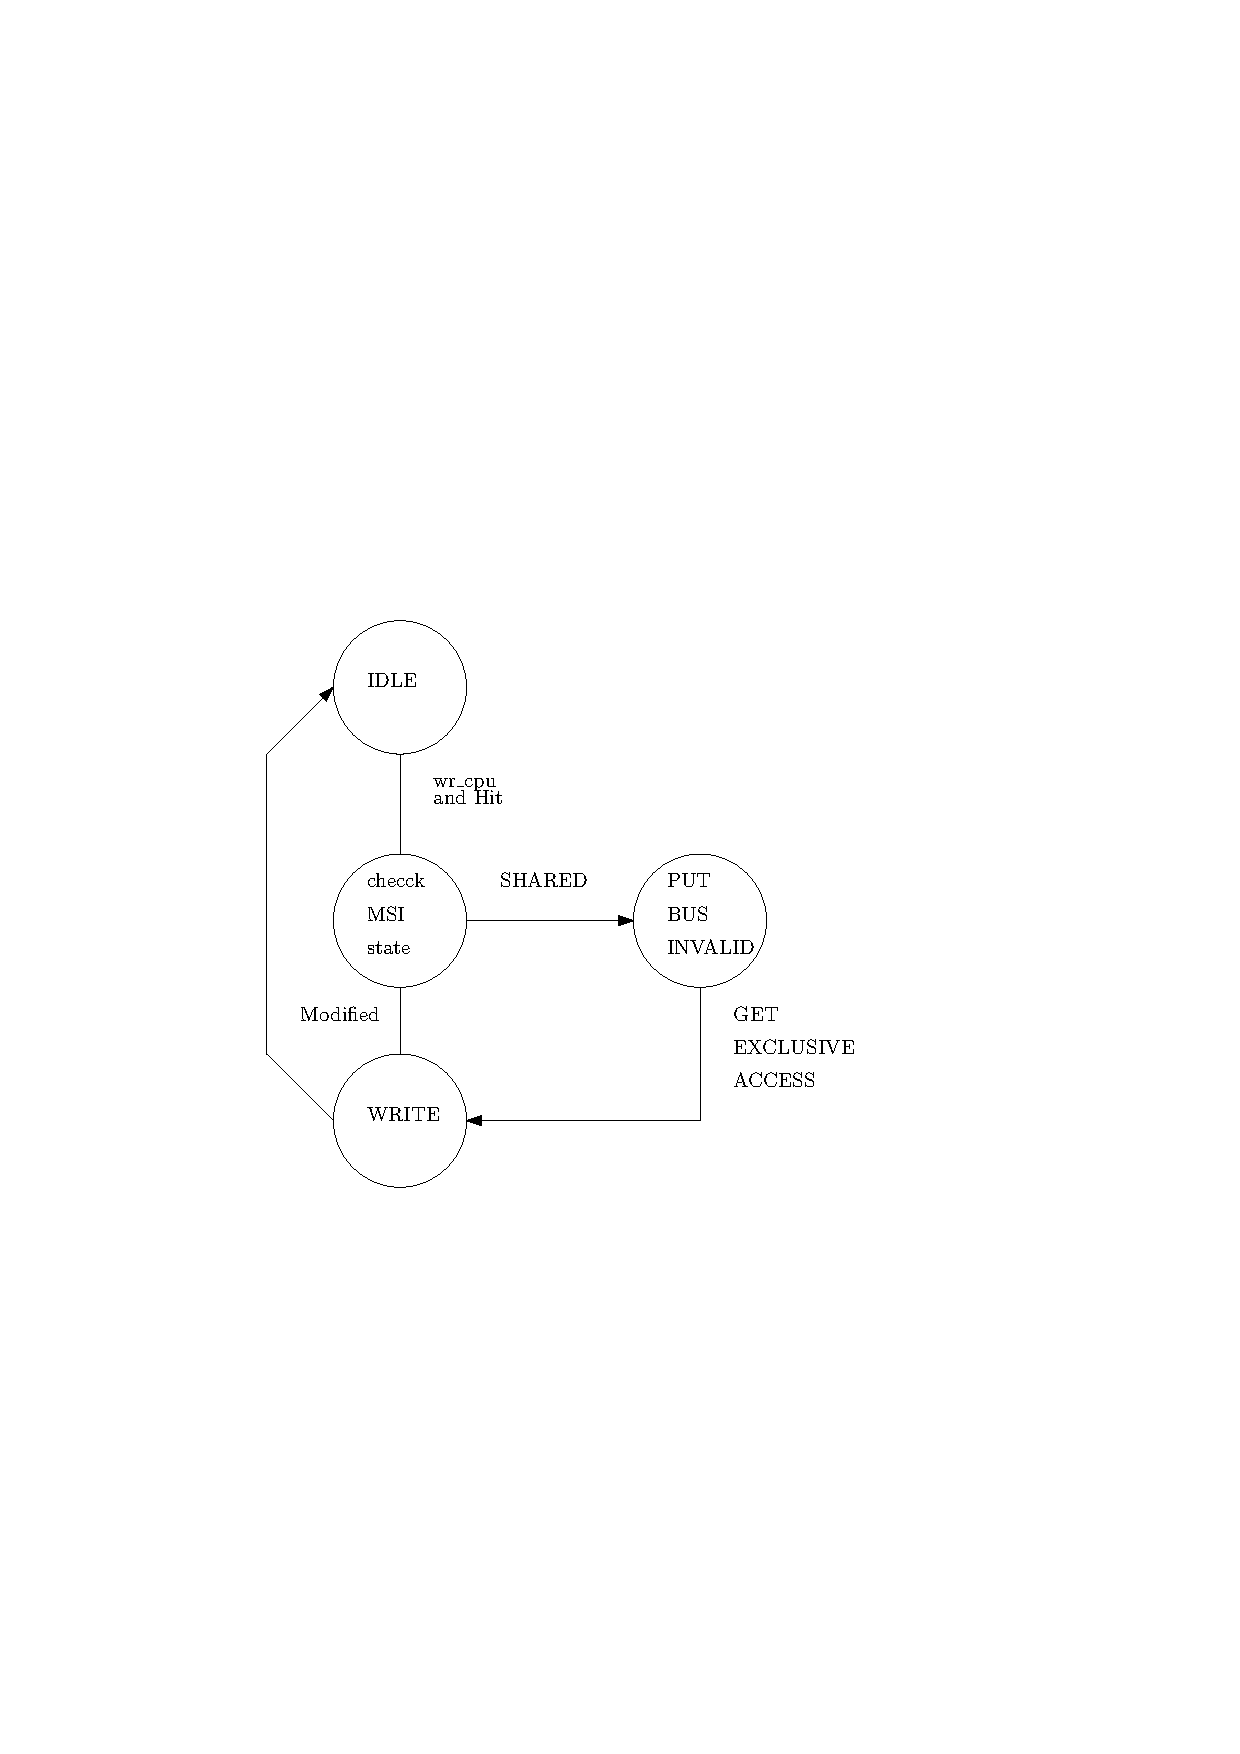
\includegraphics[width=60mm]{WRITE_INVALIPDATE.pdf}

%\vspace{-0.1in}
\caption{{\em Individual automatons}} \label{fig1}
\end{center}
\end{figure}
\end{abstract}

%\begin{IEEEkeywords}
% CyberPhysical System, \textcolor{black}{Cooperative Control}, \textcolor{black}{Code Replacement Attack}, 
% \textcolor{black}{Insider threat},  $\omega$-regular language, B\"{u}chi Automaton, Schedulability
%\end{IEEEkeywords}

%\input{introduction}

%\input{RelatedWork}
%\input{background}
%\input{Problem_statement}
%\input{Problem_statement}
%\input{Motivating_examples}
%\input{solution}
%\input{Example}
%\input{Result}
%\input{experiment}
%\input{conclusion}

%\bibliographystyle{IEEEtran}
%{\small
%\nocite{*}
%\bibliography{references}
%}
%\bibliographystyle{abbrv}
%\bibliography{main}
\end{document}
